\section{�tablir un syst�me RAID}
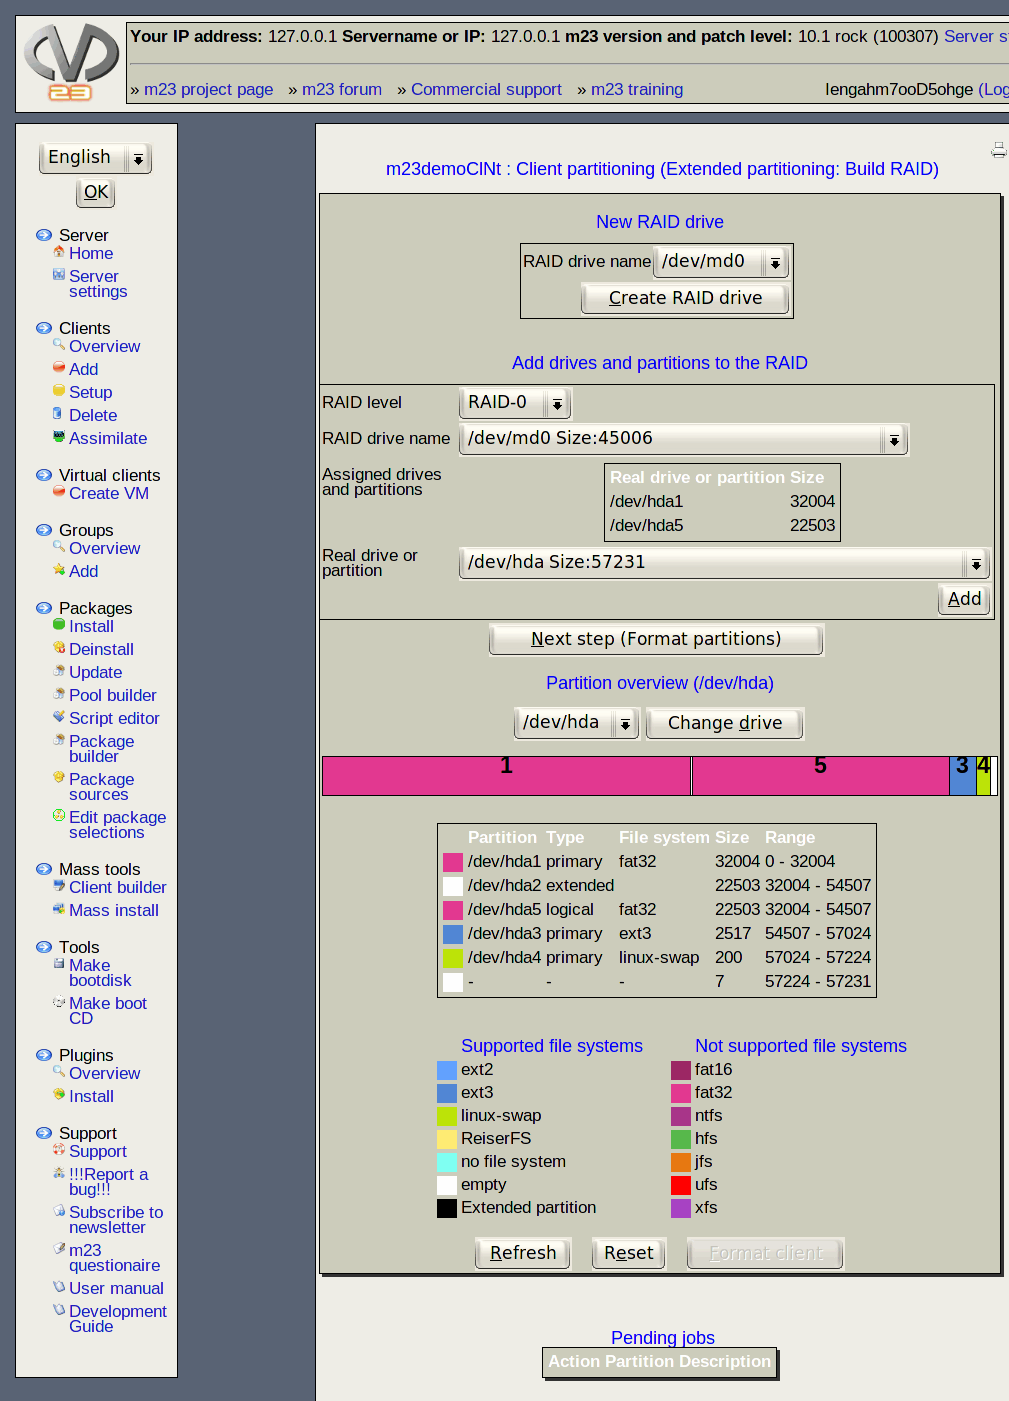
\includegraphics[scale=0.4]{/mdk/doc/manual/screenshots/fr/RAID_add.png} \\
Dans ce dialogue, vous pouvez unir des partitions ou des lecteurs entiers en forme d'un syst\`eme logique d'un RAID. m23 et le programme mdadm respectivement supportent les types de RAID 0, 1, 4, 5, 6 et 10, qui offrent des avantages et d\'esavantages diff\'erents quant \`a la augmentation de vitesse et s\'ecurit\'e de panne. Pour information suppl\'ementaire, lisez la page wikipedia http://fr.wikipedia.org/wiki/RAID_(informatique), s'il vous pla\^it. Vous pouvez \'etablir de plusieurs syst\`emes RAID par poste client et ensuite, vous pouvez utiliser les pour l'installation du syst\`eme d'exploitation, la partition swap etc. S'il vous pla\^it, lisez l'information suppl\'ementaire, quand vous voudriez installer le syst\`eme d'exploitation sur un lecteur RAID.\\
\subsection{Proc\'ed\'e \'etape par \'etape d'\'etablissement d'un syst\`eme RAID}
\begin{enumerate}
\item \textbf{\'Etablir le lecteur RAID:} S\'electionnez un nom de la liste \textit{$\ll$Nom du lecteur RAID$\gg$} et ensuite, cliquez sur \textit{$\ll$�tablir le lecteur RAID$\gg$}. Ce lecteur sera un multi-syst\`eme virtuel.\\
\item \textbf{Ajouter des partitions et des lecteurs:} Dans la case \textit{$\ll$Joindre des lecteurs et partitions au RAID$\gg$}, vous trouvez toutes les fonctions n\'ecessaires pour l'assignation des partitions ou des lecteur \`a un syst\`eme RAID. Choisissez le type du RAID et le lecteur RAID des listes correspondantes. Ensuite, vous pouvez assigner la partition ou le lecteur mentionn\'e dans la liste \textit{$\ll$Lecteur ou partition veritable$\gg$} au dessous au syst\`eme RAID par un clic sur \textit{$\ll$Ajouter$\gg$}. Dans la table \textit{$\ll$Lecteur(s)/Partition(s) assign�(e)(s)$\gg$}, vous voyez les lecteurs et partitions d\'ej\`a assign\'es.\\
\item \textbf{Terminer l'\'etablissement du syst\`eme RAID:} Ensuite, cliquez sur \textit{$\ll$Pas suivant (Formater les partitions)$\gg$}.\\
\end{enumerate}
\subsection{Informations suppl\'ementaires concernant les syst\`emes RAID et les partitions}
Les RAIDs seront acc\'ed\'es par la fonction \textit{$\ll$multi device$\gg$} du noyeau Linux. Les lecteurs RAID cr\'e\'es d'une telle fa\c{c}on se comportent comme des partitions et ne peuvent pas \^etre partitionn\'es de plus. La nouvelle variante du RAID avec possibilit\'e de partitionnement n'est pas utilis\'ee, afin de garantir la compatibilit\'e avec des noyeaux plus vieux.\\
\subsection{Information pour l'installation d'un syst�me d'exploitation sur des syst�mes RAID}
Quand le syst�me d'exploitation doit �tre install� sur un lecteur RAID, il est n�cessaire dans la plupart des cas (sauf pour RAID-1) que vous �tablissiez une partition suppl�mentaire, qui ne fait pas partie du lecteur RAID pour le noyeau et les modules. Une taille de environ 50 MB suffit pour cette partition. S'il n'y aie plus de partition libre, cliquez sur le bouton \textit{Pr�cedent} jusqu'� ce que vous atteigniez � l'�tablissement et effacement de partitions et �tablissez une petite partition.\\
